\documentclass[a4paper,12pt]{article}
\usepackage{geometry}
\geometry{left=3cm,right=1.5cm,top=2cm,bottom=2cm}
\usepackage{mathtext}
\usepackage[T2A]{fontenc}
\usepackage[russian]{babel}
\usepackage{amstext,amsmath,amssymb}
\usepackage{bm}
\usepackage[pdftex]{graphicx}
\usepackage{amsfonts}
\usepackage{indentfirst}
\usepackage{cite}
\usepackage{multirow}
\usepackage{array}
\linespread{1.3}
\pagestyle{plain}
\bibliographystyle{plain}
\begin{document}
	\begin{titlepage}
		\begin{center}
			Министерство образования и науки РФ\\
			ФГАОУ ВО Дальневосточный федеральный университет \flqq ДВФУ\frqq\\
			Школа естественных наук\\
			Кафедра компьютерных систем\\
		\end{center}
		\vspace{5cm}
		\begin{center}
			\LARGE\bf{Тема диплома}
		\end{center}
		\begin{center}\large
			Несоответствие темы диплома и текста в этом документе
		\end{center}
		\vspace{3cm}
		\large
		\begin{flushright}
			\textbf{Выполнил:}\\
			студент группы Б8117-09.03.02\\
			Махмудов Рамис Дамирович\\
			\vspace{1cm}
			\textbf{Научный руководитель:}\\
			(к.ф.-м.н.) \\
			доцент Шевченко Юрий Андреевич
		\end{flushright}
		\vspace{1cm}
		\begin{center}
			Владивосток\\2021
		\end{center}
	\end{titlepage}
	\tableofcontents
\newpage

	\newpage
	\newpage
	\section{Изображения} 
	\label{s1}
Места в Америке
	\begin{figure}[h] 
		\center{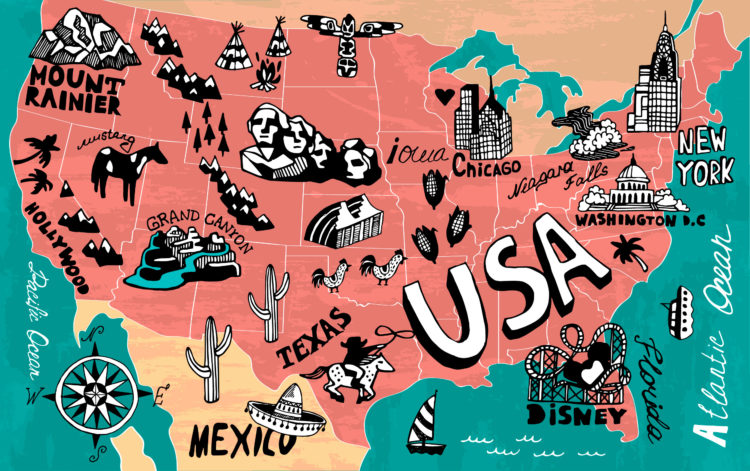
\includegraphics[scale=0.4]{1.jpg}}
		\caption{Общая карта США}
		\label{f1}
	\end{figure}
	\begin{figure}[b] 
		\center{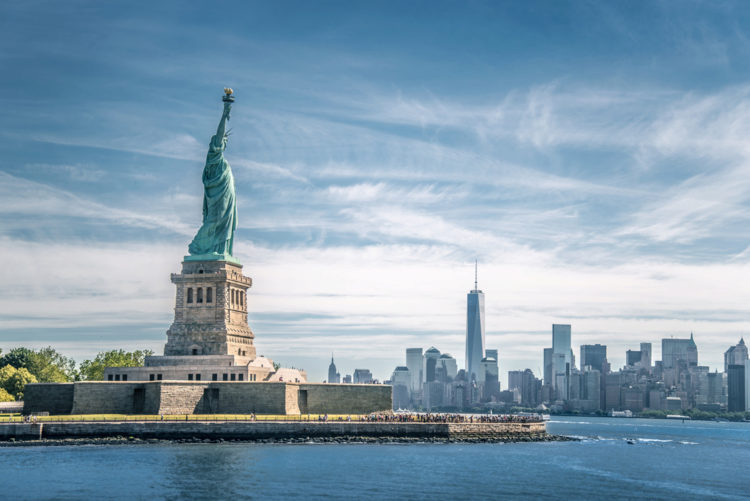
\includegraphics[scale=1]{2.jpg}}
		\caption{Статуя свободы}
		\label{f2}
	\end{figure}
Что посмотреть в США каждому приезжающему сюда туристу? Конечно, Статую Свободы и Голливудскую Аллею звезд, ответят бывалые путешественники. Но есть и еще множество интересных мест в Соединенных штатах, которые наверняка надолго останутся в памяти туриста. Мы же сделали краткий обзор, где описали основные достопримечательности США.

Впервые оказавшись в Америке, люди стремятся увидеть все достопримечательности США. Один из самых известных в мире символов страны – Статуя Свободы – расположен на небольшом острове в порту Нью-Йорка.

Величественная скульптура женщины с факелом в руке, протянутым в небеса, стала олицетворением свободы Америки. Корона на ее голове имеет семь лучей, что обозначает семь континентов и семь океанов (по западной географической традиции). В другой руке она держит плиту с выбитой на ней датой принятия Декларации о независимости. (рис.~\ref{f2}).
		\cite{SHTAB}
	\begin{figure}[t] 
		\center{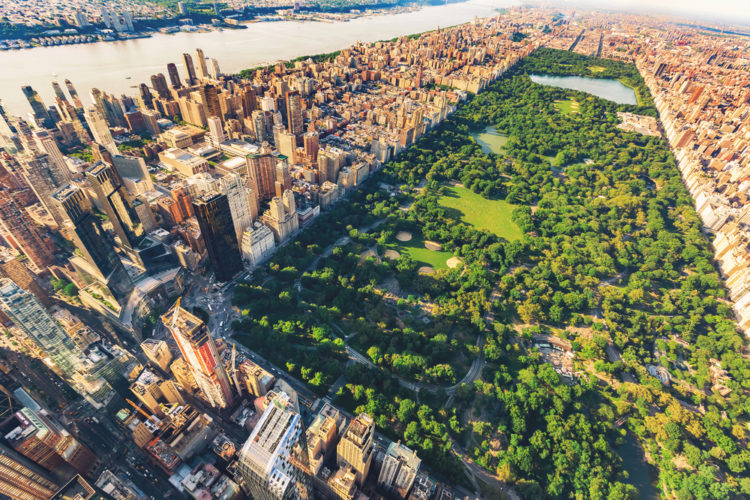
\includegraphics[scale=1]{3.png}}
		\caption{Центральный парк}
		\label{f3}
	\end{figure}
	\newpage
	\section{Уравнения, списки} 
	\label{s2}
	Достопримечательности США вызывают большой интерес у туристов. Особое место среди них занимает нью-йоркский Центральный парк. Это оазис спокойствия в бурном деловом потоке Манхэттена. Зеленая зона раскинулась на 4 км в длину и 800 метров в ширину.
	
	Открытие парка состоялось в 1859 году. Десятки тысяч рабочих еще 20 лет облагораживали территорию. Было посажено около 5 млн деревьев, а землю привозили из экологически чистых зон.
	
	Теперь парк имеет целую инфраструктуру отдыха. Это различные игровые площадки, аттракционы, катки и просто лужайки для пикника. На территории парка находятся:~\ref{f3} (раздел~\ref{s1}),
		\begin{enumerate} 
		\item Центральный зоопарк;
		\item Дайри;
		\item Гапстоу Бридж.
		\item Овечий луг.
		\item Бельведер.
		\item Сад Шекспира.
	\end{enumerate}
	\begin{eqnarray}
		\label{e1}
		\rho^2_1 = Y^2 - (Y - Z^2)^2 = \nonumber \\
		= (r_0 + \frac{\lambda}{2})^2 - (r_0 + x)^2.
	\end{eqnarray}
	уравнение~(\ref{e1}) двухстрочное. Тогда
	\begin{equation}
		\label{e2}
		x = \frac{r_0}{Y^2 + r_0}\frac{\lambda}{2}.
	\end{equation}
	Это обычные уравнения, не подходящие в текст
	\begin{equation}
		\label{e3}
		S_1 = \pi\frac{Yr_2}{Y^2 + r_2}{1-Z}\lambda.
	\end{equation}
Очередное бессмысленное уравнение
	\cite{Smik}
	\newpage
	\section{Таблицы} 
	\label{s3}
	\begin{table}[h] 
		\label{t1}
		\begin{center}
			\begin{tabular}{|c|c|c|c|}
				\hline
				Sittle & 18 september & 9:3 & 91046\\
				\hline
				Buffalo & 9 october & 19:30 & 84679\\
				\hline
				Carolina & 20 december & 10:13 & 86109\\
				\hline
				Maiami & 6 november & 10:14 & 83500\\
				\hline
			\end{tabular}
		\end{center}
		\caption{Посещаемость городов}
	\end{table}
	\newpage
\begin{figure}[h]
	\centering
	\begin{gnuplot}
		set terminal epslatex color size 12cm,15cm
		set xzeroaxis lt -1
		set yzeroaxis lt -1
		set style line 1 lt 1 lw 4 lc rgb '#4682b4' pt -1
		set grid ytics lc rgb '#555555' lw 1 lt 0
		set grid xtics lc rgb '#555555' lw 1 lt 0
		set xrange [-3:3]
		plot x**3 title '$y = x^3$' ls 1	
	\end{gnuplot}
\end{figure}
	Еще списки:
	\begin{itemize}
		\item Белый Дом;
		\item Пентагон;
		\item Здание ФБР;
		\cite{posl}
	\end{itemize}
	\newpage
	
	\section{Список литературы}
	\bibliography{mybib}
\end{document}